\chapter{Context}\label{ch:context}

\section{Voting systems}\label{sec:voting-systems}

A qualitative analysis of relevant research data reveals several critical properties of voting systems, specifically electronic ones.
For example, \textcite[section 2]{lowry_desirable_2009} name auditability, ballot secrecy, usability, incoercibility, and accessibility, while~\textcite[11-12]{jafar_blockchain_2021} add that transparency, data integrity, and participation verifiability are essential features as well.

The properties shown in~\cref{tab:properties-of-voting-systems} are most commonly mentioned in research on electronic voting systems~\autocites{agora_agora_nodate}{diaz-santiso_e-voting_2021}{jafar_blockchain_2021}{lowry_desirable_2009}{committee_of_ministers_council_of_europe_recommendation_2017}{national_democratic_institute_transparency_2013}{tas_systematic_2020}.

\begin{table}[H]
    \begin{tabularx}{\textwidth}{sCb}
        \hline
        \textbf{Property} & \textbf{Times mentioned} & \textbf{Description}  \\
        \hline
        Auditability & 4 & Election results are auditable \\
        \hline
        Anonymity & 5 & Voters are anonymous \\
        \hline
        Usability & 2 & The application is usable for a broad part of the population \\
        \hline
        Accessibility & 5 & The application is accessible and does not exclude handicapped citizens \\
        \hline
        Security & 4 & The voting process is secure and results are immutable  \\
        \hline
        Scalability & 4 & The software can handle millions of requests while also maintaining cost-efficiency \\
        \hline
        Transparency & 5 & Election processes are transparent and software is open-source  \\
        \hline
        Incoercibility & 3 & Voters can not be coerced to vote in a certain manner \\
        \hline
    \end{tabularx}
    \caption[Crucial properties of electronic voting systems]{Crucial properties of electronic voting systems}
    \label{tab:properties-of-voting-systems}
\end{table}

\section{Blockchain}\label{sec:blockchain}

Even though the first blockchain-like protocol was proposed by \textcite{chaum_computer_1982}, the concept of modern \gls{Blockchain} technology was first introduced in 2008 by \textcite{nakamoto_bitcoin_2008} and with the subsequent launch of Bitcoin in 2009.
Although Satoshi Nakamoto's real identity remains a mistery to this day, he alluded to his motivations with a message left in Bitcoin's \gls{GenesisBlock}.
It reads \enquote{The Times 03/Jan/2009 Chancellor on brink of second bailout for banks}~\autocite{nakamoto_bitcoin_2009} and refers to the headline of an article that appeared in \emph{The Times} on January 3, 2009, in the midst of the \gls{GFC} (see listing~\ref{lst:genesis-block-message}).

\codeFromFile{text}{code_snippets/genesis_block_message.sh}{Nakamoto's message in the Genesis Block}{Nakamoto's message in the Genesis Block}{lst:genesis-block-message}

A \gls{Blockchain} is a distributed ledger, meaning a decentrally updated data structure maintained by a \gls{P2P} network~\autocites[3]{crosby_blockchain_2015}[1]{nakamoto_bitcoin_2008}.
\Gls{Blockchain} protocols secure data immutability in a trustless network without the need for a central authority~\autocites[3]{crosby_blockchain_2015}[4]{jafar_blockchain_2021}.
These protocols reward nodes, also called miners, for validating and adding new data to the \gls{Blockchain} in the form of blocks that consist of bundled transactions propagated to the network by its users.
More specifically, when a sender initiates a transaction, he first signs it, then all nodes in the network receive the transaction and add it to their local blocks.
However, before they can add their block to the \gls{Blockchain}, they must solve a hash calculation looking for a hashed output that begins with a number of zero bits (see~\cref{subsec:pow}).
This operation is called \gls{POW}, as it requires energy in the form of computing power~\autocite[3]{nakamoto_bitcoin_2008}.

\subsection{Blocks}\label{subsec:blocks}

As mentioned above, the \gls{Blockchain} consists of data blocks linked to each other in a chain.
The end of the chain is the most recently mined block, so following the chain back to its start essentially means following the entire transaction history of the \gls{Blockchain} back to its first transaction in the second block.
The first block of the chain is the \gls{GenesisBlock}, which contains no transaction data as it initiates the \gls{Blockchain} when the network is deployed~\autocites[162]{antonopoulos_mastering_2017}[31]{antonopoulos_mastering_2019}.

\subsubsection{Block structure}\label{subsubsec:block-structure}

Depending on the \gls{Blockchain}, block structures might vary, though, according to~\textcite[15-16]{yaga_blockchain_2018}, the structure shown in~\cref{tab:block-structure} represents a commonly implemented data field.

\begin{table}[H]
    \begin{tabularx}{\textwidth}{ssb}
        \hline
        \textbf{Size} & \textbf{Field} & \textbf{Description} \\
        \hline
        4 bytes & Block size & The block's size in bytes excluding this field \\
        \hline
        80 bytes & Block header & Metadata \\
        \hline
        1-9 bytes & Transaction counter & Number of transactions in the block \\
        \hline
        Variable & Transactions & The transactions submitted with this block \\
        \hline
    \end{tabularx}
    \caption[Block structure]{Block structure. Note that block sizes may also vary between different \glspl{Blockchain}. Based on \textcite[160]{antonopoulos_mastering_2017}}
    \label{tab:block-structure}
\end{table}

\subsubsection{Block header}\label{subsubsec:block-header}

The block header contains metadata about the block itself and a reference to the previous block hash (see~\cref{fig:prev-block-hash}), establishing a chain link~\autocites[160]{antonopoulos_mastering_2017}[3]{nakamoto_bitcoin_2008}[15]{yaga_blockchain_2018}.
Nodes always work on bundling transactions in a new block using the latest accepted block's hash value in the block header~\autocite[3]{nakamoto_bitcoin_2008}.
Aside from the previous block's hash value, a block header contains the current timestamp, \gls{POW} difficulty target for the current block and the nonce (see~\cref{subsec:pow}), as well as the \gls{MerkleTree} root, a data structure summarizing all transactions in the block~\autocites[160-161]{antonopoulos_mastering_2017}[15-16]{yaga_blockchain_2018}.

\begin{figure}[h]
    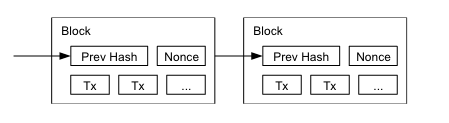
\includegraphics{nakamoto-2008-blocks}
    \caption[Linked blocks]{Linked blocks~\autocite{nakamoto_bitcoin_2008}}
    \label{fig:prev-block-hash}
\end{figure}

As \textcite[2-3]{nakamoto_bitcoin_2008} states, the inclusion of the previous block hash and the timestamp in a block's header serve a security purpose where protection grows stronger with every subsequent block added to the chain.
This is because a bad actor propagating an altered block to the network cannot do so without changing its hashed value, which would also change the next block's value as it includes the hash of its predecessor.
Thus, an attacker would first have to change the target block and then redo the \gls{POW} for all blocks that followed while outrunning the mining efforts of every honest node in the network.

\subsection{Hash algorithms}\label{subsec:hash-algorithms}

In cryptography, hashing functions are used to calculate a relatively unique fixed-length deterministic output, also called digest, from an arbitrary-length input value, as stated by~\textcite[188]{antonopoulos_mastering_2017}.
The digest acts as a digital fingerprint of the given value, meaning that individuals can verify data with hash functions independently and would immediately recognize changes to already existing data since these would produce an entirely different digest when hashed~\autocites[188-189]{antonopoulos_mastering_2017}[7]{yaga_blockchain_2018}.

\subsubsection{SHA-256}
Many \glspl{Blockchain} utilize the \gls{SHA} hash function with an output of 256 bits.
SHA-256 outputs a 32-byte hexadecimal value equaling 256 bits.
Hence, SHA-256 can produce \begin{math}2\textsuperscript{256}\approx10\textsuperscript{77}\end{math} unique digest values.

\codeFromFile{python}{code_snippets/hash.py}{Simple example of a SHA-256 hashing script in Python}{Simple example of a SHA-256 hashing script in Python}{lst:simple-example-of-sha256}

The Python script displayed in listing~\ref{lst:simple-example-of-sha256} yields the below output where the prefix \emph{0x} indicates a binary sequence will follow:

\smallskip
\begingroup\small\emph{0x64ec88ca00b268e5ba1a35678a1b5316d212f4f366b2477232534a8aeca37f3c}\endgroup
\smallskip

Since SHA-256 can produce such a high number of unique digests, it is considered collision-free, meaning it is improbable that two unique inputs will produce the same output~\autocite[8]{yaga_blockchain_2018}.

\subsection{Asymmetric key cryptography}\label{subsec:asymmetric-key-cryptography}

\Gls{Blockchain} technology relies on asymmetric key cryptography.
In asymmetric key cryptography, two keys are used, the \gls{PK} and the \gls{PBK} (see~\cref{fig:asymmetric-key}).

\begin{figure}[H]
    \begin{subfigure}[b]{\textwidth}
        \centering
        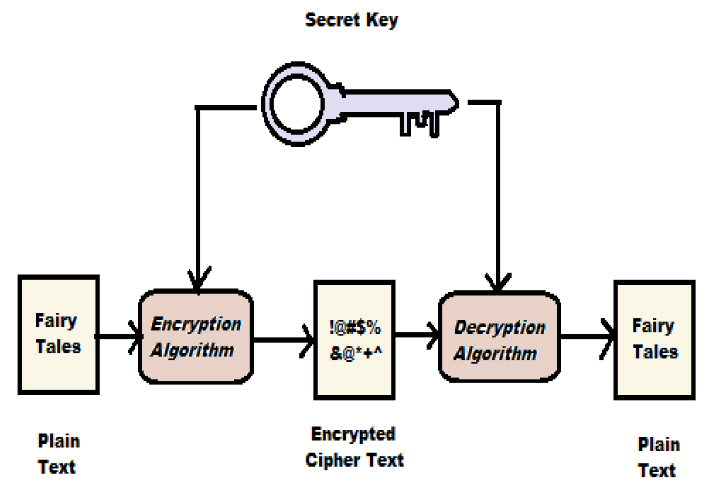
\includegraphics[scale=0.4]{chandra-2014-symmetric_key}
        \caption{Symmetric key}
        \label{fig:symmetric-key}
    \end{subfigure}
    \begin{subfigure}[b]{\textwidth}
        \centering
        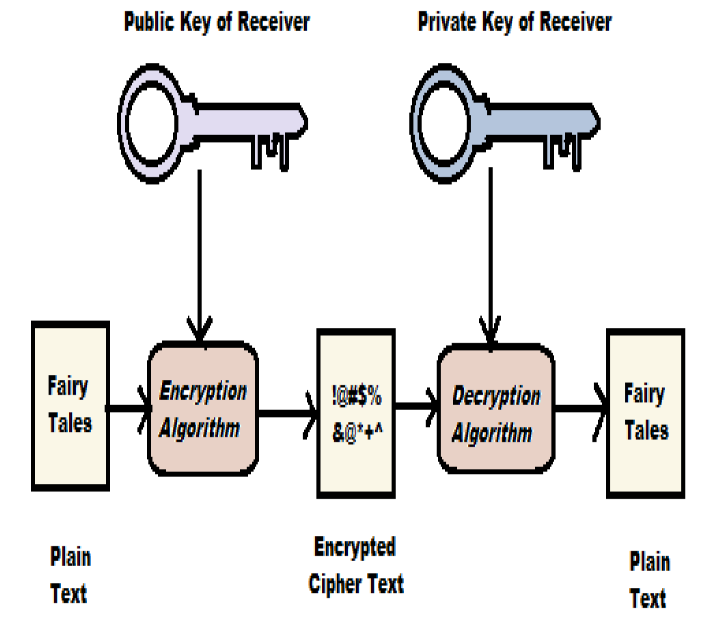
\includegraphics[scale=0.4]{chandra-2014-asymmetric_key}
        \caption{Asymmetric key}
        \label{fig:asymmetric-key}
    \end{subfigure}
    \caption[Cryptographic keys]{Cryptographic keys~\autocite[84]{chandra_comparative_2014}}\label{fig:cryptographic-keys}
\end{figure}

Contrary to symmetric key encryption shown in~\cref{fig:symmetric-key}, where both users possess the same key and are therefore required to trust each other, asymmetric key encryption demands no such trust~\autocites[84]{chandra_comparative_2014}[11]{yaga_blockchain_2018}.
This is a critical difference since users cannot trust nodes in the network and vice versa.
By employing a particular type of asymmetric key cryptography, called elliptic curve cryptography (see~\cref{subsec:elliptic-curve-cryptography}), \gls{Blockchain} users can prove ownership over funds via signing transactions with their \gls{PK} without the need to share it with untrusted third parties.
Meanwhile, nodes in the network can verify the alleged ownership using the \gls{PBK}.

\subsection{Elliptic curve cryptography}\label{subsec:elliptic-curve-cryptography}

\begin{figure}[H]
    \begin{center}
        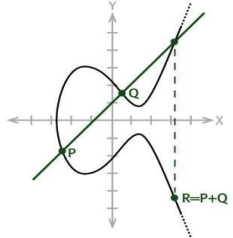
\includegraphics{kapoor-2008-elliptic_curve}
    \end{center}
    \caption[Point addition on an elliptic curve]{Point addition on an elliptic curve~\autocite[5]{kapoor_elliptic_2008}}
    \label{fig:elliptic-curve}
\end{figure}

Elliptic curve cryptography is another approach to asymmetric key cryptography that uses elliptic curves over finite fields.
It is based on the \emph{elliptic curve discrete logarithm} problem expressed by addition and multiplication on the curve's points~\autocites[65]{antonopoulos_mastering_2017}[5]{kapoor_elliptic_2008}.
The most crucial property of elliptic curves is that adding two points on the curve will yield a third point also located on the curve~\autocite[5]{kapoor_elliptic_2008}.
This addition can be described mathematically by

\begin{align}\label{eq:curve-addition}
    R(x_3,y_3)=P(x_1,y_1)+Q(x_2,y_2)
\end{align}

As shown in \cref{fig:elliptic-curve}, the third point is calculated geometrically by drawing a line between $P$ and $Q$, which intersects the curve at an additional point reflecting $R$ on the x-axis.

With a defined addition rule, curve multiplication can be applied with $kP$ where $k$ is a positive integer and $P$ a point on the curve as the sum of $k$ times $P$~\autocite[5]{kapoor_elliptic_2008}.

In consequence,~\textcites[65,68]{antonopoulos_mastering_2017}[5]{kapoor_elliptic_2008} state that given an agreed-upon curve \emph{generator point} $P$ and a none-secret elliptic curve, one can select a secret random integer $k$ to derive a public curve point $K$ from it using elliptic curve multiplication

\begin{align}\label{eq:curve-multiplication}
    K=k \cdot P
\end{align}

Reversing the multiplication process by solving for $k$ would be an unfeasible operation since the multiplication is nonlinear, as the output point can be anywhere on the curve with respect to the input point~\autocite{price_bitcoins_2020}.
Furthermore, going backward, i.e., solving for $P$ provided $kP$, where $k$ is a random integer, is more difficult due to the symmetry of elliptic curves.
Meaning, multiple points $P$ might exist whose tangent lines cross the negation of $kP$ for any number of additive iterations in the multiplication process (see \cref{fig:finding-point-p}).
Therefore, a sufficiently high curve order exponentially increases the computing power needed to solve for $k$, making $K$ sharable with untrusted third parties without having to sacrifice the privacy of $k$.

\begin{figure}[H]
    \begin{center}
        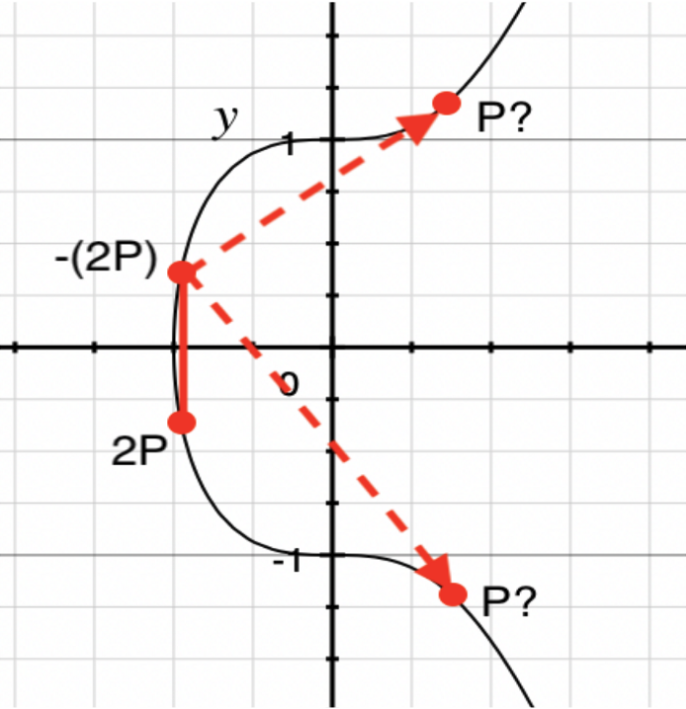
\includegraphics[scale=0.3]{price-2020-inverse-curve-addition}
    \end{center}
    \caption[Finding point $P$ in $kP$ given $k=2$]{Finding point $P$ in $kP$ given $k=2$.
    Shows the possibility of multiple points whose tangent lines cross the negation of a given point~\autocite{price_bitcoins_2020}}
    \label{fig:finding-point-p}
\end{figure}

\subsubsection{Private key}\label{subsubsec:private-key}

The \gls{PK} or $k$ (see~\cref{fig:elliptic-curve-trapdoor}) is a 256-bit number picked at random when a user creates a new wallet address;
it can be any number between $1$ and $n-1$, where $n$ is a constant that defines the order of the elliptic curve $k$~\autocite[63]{antonopoulos_mastering_2017}.

\begin{figure}[H]
    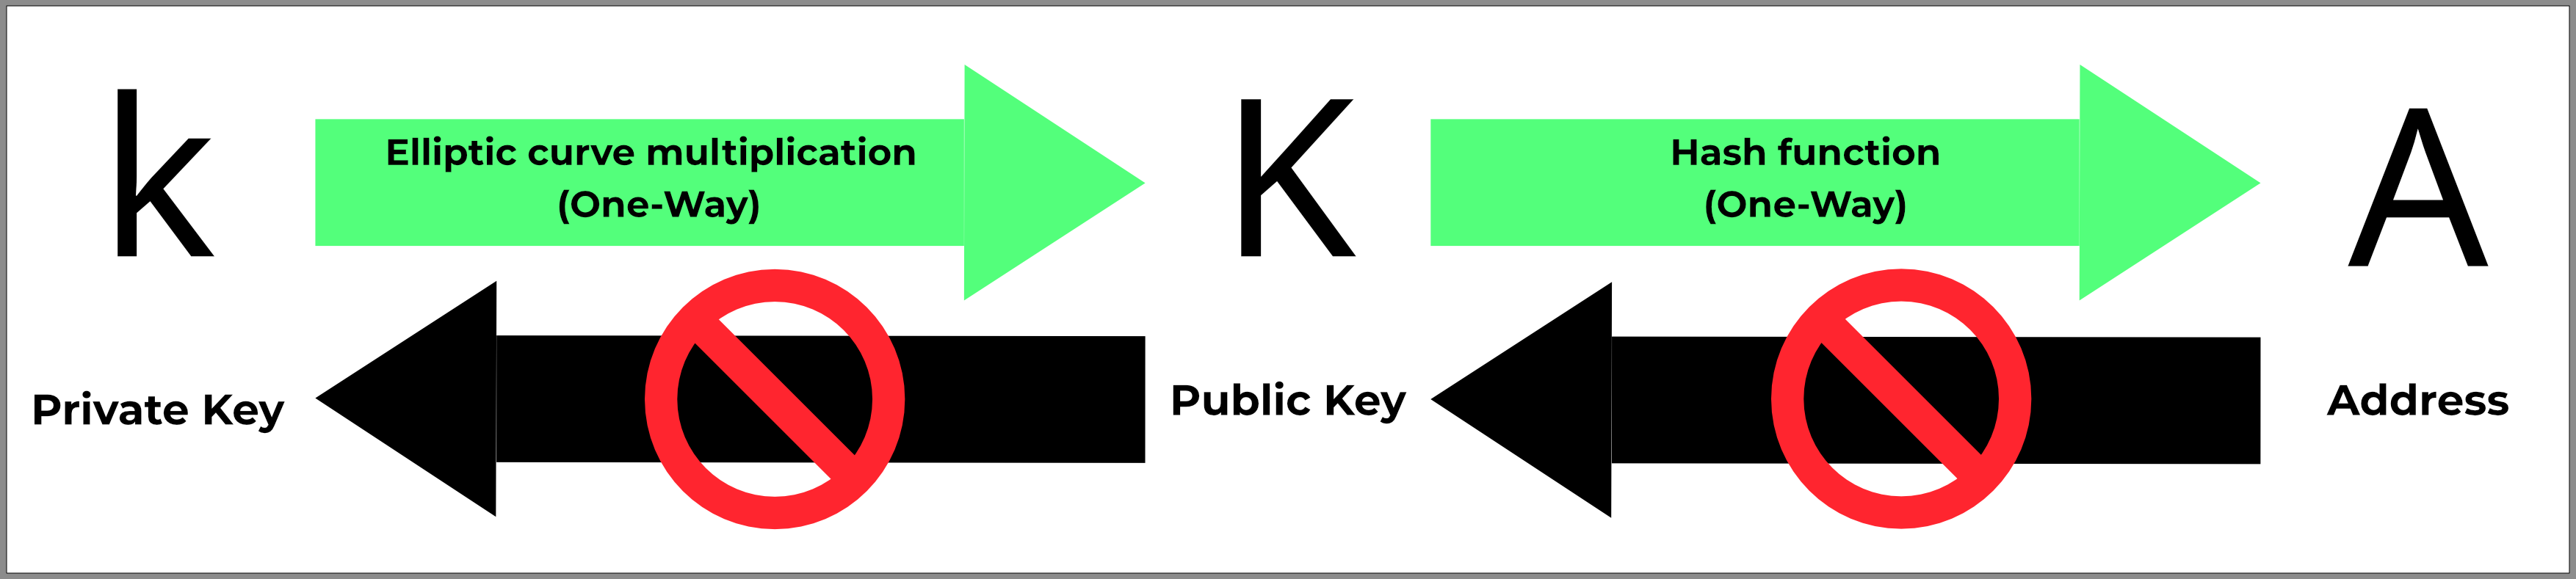
\includegraphics[width=\textwidth]{boehm-cryptographic_trapdoor}
    \caption[Cryptographic trapdoor functions]{Cryptographic trapdoor functions. Shows the direction in which trapdoor functions are utilized to achieve a one-way relationship between \gls{PK}, \gls{PBK} and a wallet's address. Based on~\textcite[160]{antonopoulos_mastering_2017}}
    \label{fig:elliptic-curve-trapdoor}
\end{figure}

\subsubsection{Public key}\label{subsubsec:public-key}

As stated above, the \gls{PBK} is generated from the \gls{PK} with elliptic curve multiplication.
The relationship between the pair is fixed and can only be calculated in one direction (see \cref{fig:elliptic-curve-trapdoor}).

\subsection{Proof of work}\label{subsec:pow}

Nodes in the network are only allowed to add a new block to the chain when they have solved a computing problem, i.e., they have to provide \glsfirst{POW}.
In the case of Bitcoin, this problem involves scanning for a value whose hashed output begins with a number of zero bits by incrementing on a \gls{Nonce}~\autocite[3]{nakamoto_bitcoin_2008}.
Furthermore, since hashing algorithms are designed to (see \cref{subsec:hash-algorithms}) produce unique outputs for a given input, aside from trying random inputs, it is also impossible to produce the desired output from a selected input~\autocite[189]{antonopoulos_mastering_2017}.

\codeFromFile{python}{code_snippets/hash_nonce.py}{Iterating on a nonce. Based on~\textcite[189]{antonopoulos_mastering_2017}}{Iterating on a nonce}{lst:hashing-script-with-nonce}

Listing~\ref{lst:hashing-script-with-nonce} illustrates a simplified hashing function that will output different hashes by adding a \gls{Nonce} to the input value on each iteration.
For instance, if the difficulty target is given as

\smallskip
\begingroup\small\emph{0x0010000000000000000000000000000000000000000000000000000000000000}\endgroup
\smallskip

a smaller hash would need to start with three zero bytes.
The winning \gls{Nonce} in this example would then be 11 (see listing~\ref{lst:output-of-hashing-script}).
Hence, the act of finding the winning \gls{Nonce} would be \gls{POW} equivalent to the computing power needed to run this script 12 times.

\codeFromFile{text}{code_snippets/hash_output.sh}{Output of hashing script iterating on a nonce}{Output of hashing script iterating on a nonce}{lst:output-of-hashing-script}

Clearly, \gls{POW} hashing algorithms employed by \gls{Blockchain} protocols are considerably more complex but in principle this is how they work.
Consequently, once a node has provided the \gls{POW} required by the network to add a new block to the chain an attacker would need to redo the work for that block and all subsequent blocks in order to manipulate data.

\subsection{Proof of stake}\label{subsec:pos}

\Gls{POS} is another consensus mechanism that moves the decision basis from energy consumption to the possession of funds, i.e., a stake in the network~\autocites[321]{antonopoulos_mastering_2019}[chapter 1]{udokwu_state_2018}[3]{udokwu_evaluation_2020}.
Similarly to \gls{POW}, anyone can become a validator provided they are willing to make the necessary investment.
A \gls{POS} network utilizes an algorithm that selects validators randomly from a pool of staked deposits~\autocite[3]{udokwu_evaluation_2020}.
Validators then take turns proposing and voting on the next block while their voting power is determined by the amount of their deposit~\autocite[321]{antonopoulos_mastering_2019}.
Since validators risk losing their staked deposit if the network rejects their block, they are incentivized to act honestly~\autocite[321]{antonopoulos_mastering_2019}.

\section{Web3}\label{sec:web3}

\Gls{Web3} commonly refers to the third version of the internet, signifying a move from centralized to decentralized applications~\autocite[xxxv]{antonopoulos_mastering_2019}.
A push towards decentralization of the internet is seen by many as the solution to problems associated with \gls{Web2}~\autocite{feiner_prominent_nodate}.

\subsection{Ethereum}\label{subsec:ethereum}

Shortly after Nakamoto launched Bitcoin, developers started to realize the potential of the underlying technology and began trying to apply it to applications in general.
However, Bitcoin's constraints meant that applications built on top of its protocol were very limited in what they could do~\autocite[3]{antonopoulos_mastering_2019}.
Therefore, the development of a new \gls{Blockchain} that combines Bitcoin's technology with a general-purpose computing architecture seemed to be the only feasible option~\autocite[3]{antonopoulos_mastering_2019}.
Such a \gls{Blockchain} was proposed by Vitalik Buterin in~\citeyear{buterin_ethereum_2014} and became known as Ethereum.
It was the first \gls{Blockchain} offering a built-in Turing-complete programming language~\autocite[13]{buterin_ethereum_2014}.

\subsection{Turing completeness}\label{subsec:turing-completeness}

The term is a reference to Alan Turing who defined a mathematical model of a computational system that manipulates states by reading and writing on sequential memory.
In computability theory Turing's model is the basis for answering questions about universal computability, where a system is said to be Turing-complete if it can simulate any Turing machine~\autocite[8]{antonopoulos_mastering_2019}.
The Ethereum Virtual Machine is such a Turing-complete system, which means \glsplural{SmartContract} deployed on Ethereum can solve any computational problem regular computers can, making Ethereum a \enquote{world-computer operating under consensus}~\autocite[6]{antonopoulos_mastering_2019}.

\subsection{Comparison of Turing-complete blockchains}\label{subsec:comparison-of-turing-complete-blockchains}

Until recently, Ethereum applied a \gls{POW} consensus mechanism similar to Bitcoin's.
However, to address the issue of rising energy consumption and scalability, the Ethereum Foundation has long been planning to migrate the network to a \gls{POS} consensus layer (see~\cref{tab:comparison-of-turing-complete-blockchains}).
This has been dubbed \emph{The Merge} and was finalized on September 15, 2022~\autocite{ethereum_foundation_merge_nodate}.
Although \emph{The Merge} has reduced Ethereum's energy consumption by ~99.95\%~\autocite{ethereum_foundation_merge_nodate}, transaction speeds have not noticeably improved post-migration.

\begin{table}[H]
    \begin{tabularx}{\textwidth}{ssssss}
        \hline
        \textbf{Blockchain} & \textbf{Consensus} & \textbf{Layer} & \textbf{TPS \newline (recorded)} & \textbf{TPS \newline (theoretical)} & \textbf{Permission} \\
        \hline
        Ethereum & \gls{POS} & Layer 1 & ~50 & ~120 & permissionless  \\
        \hline
        Hyperledger Fabric & \gls{PBFT} & Layer 1 & ~13,000 & ~100,000 & permissioned \\
        \hline
        Polygon & \gls{POS} & Layer 2 & ~7000 & ~65,000 & permissionless \\
        \hline
        Solana & \gls{POH} & Layer 1 & ~3000 & ~710,000 & permissionless  \\
        \hline
    \end{tabularx}
    \caption{Comparison of turing-complete blockchains}
    \label{tab:comparison-of-turing-complete-blockchains}
\end{table}

As seen in~\cref{tab:comparison-of-turing-complete-blockchains}, Layer 2 \glspl{Blockchain} running on Ethereum's mainnet, like Polygon, are still significantly faster, theoretically scaling up to ~65,000 \gls{TPS}~\autocite{bybit_learn_11_2022}.
Conversely, Solana has the most significant scaling potential~\autocite{bybit_learn_11_2022} due to its \glsfirst{POH} consensus mechanism~\autocite{yakovenko_proof_2020}.
Nevertheless, this also means that the network is prone to downtimes and denial of service attacks, as \gls{POH} and Solana's low transaction costs provide no safeguard against spamming by bots or potential attackers.
Likewise, Hyperledger too compromises on security to achieve higher \gls{TPS} by utilizing another consensus mechanism called \glsfirst{PBFT}.
More specifically, Hyperledger enables developers to build permissioned \gls{Blockchain} networks where nodes operate under the assumption that less than one-third of their peers are faulty~\autocites{ferris_does_2019}[1]{sukhwani_performance_2017}.

\section{Development tools}\label{sec:development-tools}

\subsection{Node.js}\label{subsec:node.js}

Node.js is a JavaScript runtime environment that enables the execution of JavaScript code outside a web browser.
It is designed to build scalable network applications solely relying on JavaScript.

Node.js achieves high scalability by utilizing non-blocking asynchronous \gls{IO} with event loops~\autocites{openjs_foundation_about_nodate}[74]{shah_nodejs_2017}, enabling it to handle thousands of requests concurrently.
In contrast, conventional web servers, which handle multiple concurrent requests by creating new threads, might quickly max out the memory available to the system~\autocite[7-8]{chhetri_comparative_2016}.
In this regard, Node.js is similar to event machines built for other languages like \emph{Twisted} for Python, Ruby's \emph{Event Machine}, or \emph{MINA}, Apache's network framework library.
However, it utilizes the concept of an event loop as a runtime construct rather than a library~\autocite{openjs_foundation_about_nodate}.

\subsection{Nx}\label{subsec:nx}

Nx is a build system that provides monorepo support, thus making it possible to manage code bases for several projects in a single repository.
According to~\textcite[80]{potvin_why_2016}, this is a concept Google, whose monolith repository contains over two billion lines of code, has been embracing for over two decades.
In doing so, Google has unified versioning and simplified dependency management for its developers while encouraging code sharing across multiple applications and teams~\autocite[84]{potvin_why_2016}.
However, whereas Google has developed its own tools for managing code bases of that size in one repository, smaller companies and freelance developers can still leverage the advantages of monorepos while alleviating disadvantages with build systems like Nx or Turborepo.

As seen in listing~\ref{lst:nx-workspace}, the folder structure of a nx workspace initiated with \emph{npx create-nx-workspace@latest} looks very similar to a single project repository.
A noteworthy difference is the fact that applications and libraries have their respective root subdirectories in the \emph{libs/} and \emph{apps/} folders while still maintaining shared dependency information in the project root's package.json.
Accordingly, node modules are also installed in the root directory but nx makes them accessible across all applications and libraries in the repository.

\codeFromFile[breakable=false]{text}{code_snippets/nx_workspace.txt}{Creating a nx workspace with a React application}{Creating a nx workspace with a React application}{lst:nx-workspace}

\subsection{Next.js}\label{subsec:next.js}

Next.js is a frontend framework that utilizes React.js with added capabilities for server-side rendering of static web applications.
This means developers can write React components in Java- or TypeScript without exposing code executed on the server to the client.
However, it should be noted that the JavaScript code in React components is still executed in the browser, meaning the client will have access.

\subsubsection{JSX}\label{subsubsec:jsx}

In contrast to other frontend frameworks such as Vue.js, React does not rely on traditional \gls{HTML} syntax for the creation of elements in the document.
Instead, it uses a syntax extension called \gls{JSX}~\autocite{meta_platforms_inc_react_2022}.
\gls{JSX} provides element attributes that map to those of \gls{HTML} elements (see listing~\ref{lst:jsx}).

\codeFromFile{jsx}{code_snippets/jsx.tsx}{h1 element written in JSX}{h1 element written in JSX}{lst:jsx}

\subsubsection{States}\label{subsubsec:states}

React component states are JavaScript objects that hold data developers ultimately wish to display on the screen.
Their most important feature is that updated states trigger re-renders in the application, making the webpage dynamic~\autocite{meta_platforms_inc_react_2022}.
In modern React applications component states can be defined with the \emph{useState} hook (see listing~\ref{lst:states}).

\codeFromFile{jsx}{code_snippets/states.tsx}{Defining a React state}{Defining a React state}{lst:states}

\subsubsection{Props}\label{subsubsec:props}

Modern React applications usually embrace the concept of splitting up code by utilizing functional components.
Functional components accept \glspl{prop} as parameters, making them dynamic and reusable in other components.
This way, developers can import components in other react components, make logic decisions in the parent component and parse mutated data to the child component or vice versa.
Listing~\ref{lst:props} shows a simplified example of this where a state defined in the \emph{App} component is rendered with an initial value while a \emph{setState} function is parsed to an input element in the child component as a \gls{prop}.

\codeFromFile{jsx}{code_snippets/props.tsx}{Parsing props to subcomponents}{Parsing props to subcomponents}{lst:props}

\subsection{Nest.js}\label{subsec:nest.js}

Nest.js is regularly mentioned among the best Node.js backend frameworks~\autocites{clever_solution_9_2020}{labay_10_2020}{patel_top_2022} due to its many development features and usage of Express.js~\autocite{mysliwiec_documentation_nodate}, which is another highly regarded backend framework known for its speed.
It is specifically designed for building scalable Node.js backend applications~\autocite{mysliwiec_documentation_nodate} and utilizes design methods common among traditional backends written in languages like Java.
Accordingly, Nest.js combines elements of \gls{OOP} and \gls{FP}~\autocite{mysliwiec_documentation_nodate}.

\subsection{PostgreSQL}\label{subsec:postgresql}

PostgreSQL is an \gls{ORDBMS} first developed by researchers at the University of California, Berkeley~\autocite[3]{worsley_practical_2002}.
It is an open-source project and thus free to download and use, although there are commercially developed products based on PostgreSQL, such as Red Hat.

\subsection{Remix IDE}\label{subsec:remix-ide}

The Remix \gls{IDE} is an open-source tool for writing, debugging, and deploying \glsplural{SmartContract} on supported blockchain networks.
According to \textcite{remix_project_welcome_nodate}, some features of their \gls{IDE} are:

\begin{enumerate}
    \item A code editor with syntax highlighting and autocomplete features for Solidity
    \item A debugger that enables developers to step through state changes triggered by transactions
    \item Deployment tools enabling developers to connect their wallets and deploy their contracts on main- or testnets.
\end{enumerate}

\subsection{Hardhat}\label{subsec:hardhat}

Hardhat is a \gls{CLI} tool that provides similar features as the Remix \gls{IDE} (see \cref{subsec:remix-ide}) but is used for local development of \glsplural{SmartContract}~\autocite{hardhat_documentation_nodate}.
For more advanced use cases, developers may write and test their contracts locally, as one of Hardhat's most important features is its extensibility.